\section{Classifiers, Reduction of the dimensionality algorithms and Cross Validation}
Classifying is called to the task of assign a category to an object. The classification task is based in the obtained features of the object and the characteristics of the feature extractor \cite{Duda}. The particular case of this thesis, features obtained at the output of a Convolutional Neural Network are utilized for classification.\\

The output of the convolutional neural network could be bigger enough and some features could not be relevant for the classification. To solve the speed and robustness issues that could appear because of the quantity of features \cite{PCAvsLDA}, techniques to reduce the dimensionality are used.\\

Classifiers must be customized to each problem, to find the optimal parameters for each occasion, cross validation technique has been used.\\

\subsection{Classifiers}
In this section, the classifiers used along the thesis are described.\\

\subsubsection{Logistic Regression}
Logistic regression is a probabilistic and a linear classifier. It is customized by a weight matrix \textit{W} and a bias vector \textit{b}.\\

The logistic regression weights and bias define a linear hyperplane which is the decision boundary of the classes. In order to find the parameters, the Maximum likelihood estimation is used during training \cite{ClassifiersReview}:\\

\begin{equation}
\prod_{i=1}^{n}P(y_i|X_i,W,b)
\end{equation}

Given an input vector \textit{x}, which belongs to the \textit{i} class (a value of a stochastic variable \textit{Y}), its probability could be described as follows:

\begin{equation}
P(Y=i|x,W,b) = \frac{e^{W_ix+b_i}}{\sum_j e^{W_ix+b_i}}
\end{equation}

The class of a new sample (\textit{y\_{pred}}) would be classified as:

\begin{equation}
y_{pred} = argmax_{i}P(y_i|X_i,W,b)
\end{equation}

A sample would belong to a class depending on position in the space with respect to the hyperplane that separates the classes.\\

\subsubsection{Support Vector Machine}
Support Vector Machine (SVM) is a two-class (bi-class) classifier. The smallest generalization error is linked to the \textit{margin} concept. Margin is the perpendicular distance between the closest sample of the database and the calculate hyperplane \cite{MachineLearning}. An hyperplane is optimal if the margin is the maximum and this margin is calculated (as the same way as logistic regression):\\

\begin{equation}
\underset{w b}{\operatorname{arg\,max}}\left \{ \frac{1}{||W||} \underset{n}{\operatorname{min}}[t_{n}(W^T \phi (X_n)+b)]   \right \}
\end{equation}


Where \textit{w, b} are the parameters that should be optimized in order to maximize the distance. \textit{$t_n$} are the training samples. $\phi$ is a fixed feature-space transformation, \textit{b} is the bias parameter.\\

\begin{figure}[htb]
\centering
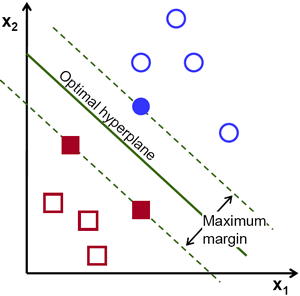
\includegraphics[width=0.5\textwidth]{images_miscelaneus/svm.png}
\caption{Optimal hyperplane and the decision boundary. Image obtained from \cite{SVMimage}} \label{fig:SVM}
\end{figure}

In figure \ref{fig:SVM} the optimal hyperplane between two classes are represented with its corresponding margin. In the given example, the two classes are well differentiated. Figure \ref{fig:SVM} has been obtained from \cite{SVMimage}.\\

Based on estimate the hyperplane that maximize the distance between classes, the closest vectors of each class are selected \cite{SVM1, MachineLearning}. In practice, the margin is determined by \textit{C}, a parameter that should be chosen by user to get the optimal margin.\\

The SVM performance is join to a kernel function which allows variability in nonlinearity and flexibility in the model \cite{ClassifiersReview, practicalguideSVM}. There are various kernels (polynomial, sigmoid, etc.), two of them are utilized:

\begin{enumerate}
\item Linear kernel: $ K(x_{i},x_{j}) = x_i^T x_j$.
\item Radial basis function (RBF) kernel: $K(x_{i},x_{j}) = exp(-\gamma||x_i-x_j||^2), \gamma>0$
\end{enumerate}

\subsubsection{K Nearest Neighbours}
K- Nearest Neighbour (KNN) is a generative and non parametric classifier. For classifying, the density estimation procedure is utilized. The difference between this classifier and others is that data is used in this algorithm directly for classification, without building a model first \cite{ClassifiersReview}. The density function is determined by the form \cite{MachineLearning}:
\begin{equation}
p(x) = \frac{K}{N V}
\end{equation}

Where \textit{K} is the number of points inside the region \textit{R} whose volume is \textit{V} and \textit{N} is the number of total samples or observations.\\

This classifier uses the observation directly to classify and needs all the samples to predict a new one. The probability of a sample \textit{x} belonging to a class \textit{$C_k$} is defined by \cite{MachineLearning}:
\begin{equation}
p(x|C_k) = \frac{K_k}{N_k V}
\end{equation}

Where $N_k$ are the observations of a class $C_k$ and $K_k$ of it class points are contained in the volume \textit{V}.\\

The \textit{K} value is fixed and constant, it should be calculated and optimized by user of each application.\\

\subsubsection{Decision Tree}
Decision Tree classifier is based in a natural classification based in a sequence of true/false or yes/no questions \cite{Duda}. It could be used as a binary classifier or a \textit{k} classes classifier. \\

The input data is split to maximize its separation, resulting a tree structure \cite{ClassifiersReview} as is described in figure \ref{fig:Tree} (image obtained from \cite{Treeimage}). Where depending on the features, a sample changes from a principal branch to a branch of this until a class is signed. The last branches correspond to the classes and the same class could be in different final branches. \\

\begin{figure}[htb]
\centering
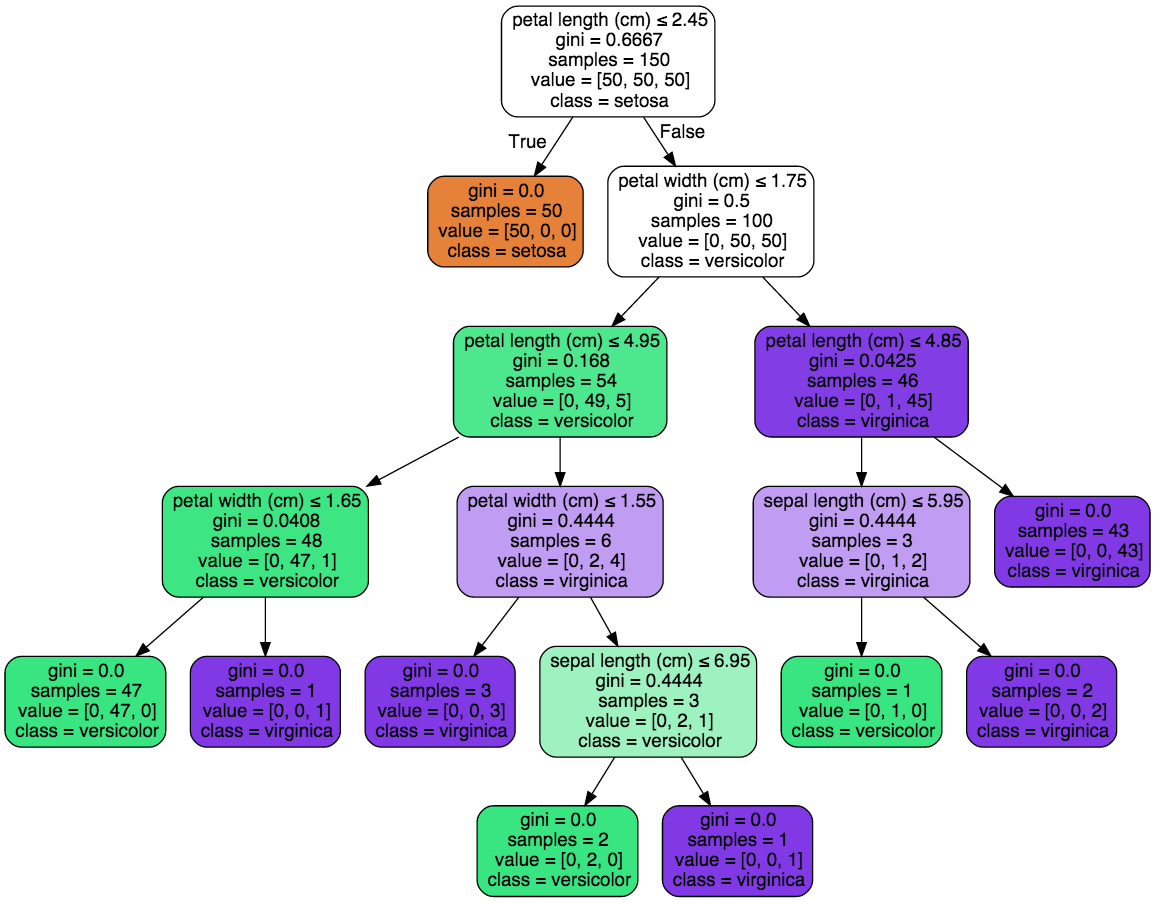
\includegraphics[width=0.55\textwidth]{images_miscelaneus/tree.png}
\caption{Decision Tree Classifier. Image obtained from \cite{Treeimage}} \label{fig:Tree}
\end{figure}

\subsection{Dimensionality reduction algorithms}
The objective of those algorithms is transformed by the characteristic vector into another characteristic vector but with a lower dimensionality. Linear methods, that projects the dimensional data onto another space whose dimensionality is lower \cite{Duda}, have been used. The two techniques, the most common used, are described and used along the thesis.\\

\subsubsection{Linear Discriminant Analysis}
Linear Discriminant Analysis (LDA) looks for the vectors in the space that best discriminate among classes, that is that LDA pretend to maximize the between-class measure (equation \ref{eq:Sb}) at the same time as the within-class measure (equation \ref{eq:Sw}) is minimized \cite{PCAvsLDA}.\\

\begin{equation}
S_w = \sum^c_{j=1}(\mu _j - \mu)(\mu _j - \mu)^T
\end{equation}\label{eq:Sb}

\begin{equation}
S_w = \sum^c_{j=1}\sum^{N_j}_{i=1}(X_i^j - \mu _j)(X_i^j - \mu _j)^T
\end{equation}\label{eq:Sw}

The data of \textit{d} dimensions would be projected onto a \textit{s} dimensions and being $s < d$. The minimum value that \textit{s} could take would depend on the number of classes \textit{n}: $s \geq n-1$.


\subsubsection{Principal Component Analysis}
Principal Component Analysis (PCA) uses a subspace \textit{t} in which the the variance direction among basis vectors is maximum in the original space \textit{f} \cite{PCAvsLDA}. PCA faces the problem of reducing the \textit{n} dimensional samples vector to a single vector $X_0$. The $X_0$ vector would be the result of the sum of the squared distances between $X_0$ and various features $X_k$ is the smallest \cite{Duda}.\\

The new subspace is usually smaller than the original space \cite{PCAvsLDA}.\\

The linear transformation from one space into another would be denoted as \textit{W}, and its columns are eigenvalues which has eigenvectors associated.\\

The feature vectors (\textit{y}) from the \textit{f} space would depend on W:

\begin{equation}
y_{i} = W^TX_{i}, i=1,...,N
\end{equation}

Being N the total number of feature vectors.\\

\subsection{Cross Validation}
Classifiers are defined by certain parameters. For example,the number of neighbours (\textit{k}) in KNN classifier is a value that user have to determine. In this case is useful use Cross Validation to determine the value of \textit{k}.\\

This method uses the training samples. They are split in groups (\textit{kfolds}) and used to train and test the classifier with different values; in the KNN case, the value k would be change. A metric (score) is calculated and it is possible to determine the value of the classifier in which the metric is the optimum.\\

This technique has been use to calculate the value which a classifier is defined. For SVM classifier the value \textit{C}, for KNN classifier the value {k}, for Decision Tree classifier the depth of the tree, softmax classifier to determine the learning rate when it has not been trained at the same time of the network and for PCA and LDA the number of components. \\
